\chapter{Discesa del gradiente}
\section{L’uso delle reti neurali per riconoscere caratteri scritti a mano}
Seppure la maggior parte delle persone riconosce facilmente le cifre scritte a mano 504192, la facilità di questo processo è estremamente ingannevole per due motivi:
\begin{itemize}
    \item In ogni emisfero del nostro cervello abbiamo una corteccia di visualizzazione primaria (chiamata V1) contenente circa 140 milioni di neuroni e miliardi di connessioni.
    \item Oltre alla V1 è presente un’intera serie di cortecce di visualizzazione (V2, V3, V4 e V5) le quali svolgono un processing completo dell’immagine in maniera progressiva.
\end{itemize}
\begin{figure}[!h]
    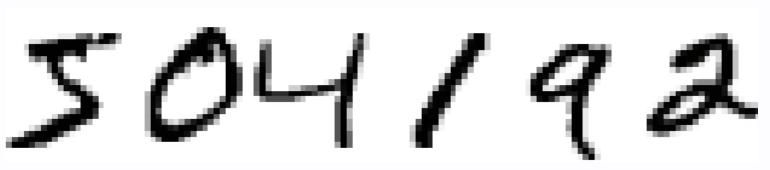
\includegraphics[scale=.5]{images/gradient_descent/digit.png}
    \centering
\end{figure}




Proprio per questo motivo il riconoscimento di caratteri scritti a mano non è un processo semplice.
La difficoltà del visual pattern recognition diventa evidente se si cerca di realizzare un codice in grado di riconoscere le cifre come quelle mostrate nell’esempio precedente. Difatti ci sono semplici elementi che ci permettono di comprendere la cifra che non sono semplici da esprimere algoritmicamente. Ad esempio noi sappiamo che il numero 9 è formato da un cerchio posto in alto ed una linea dritta in basso a destra. Proprio questi elementi sono molto complessi da esprimere mediante un algoritmo. 
Il machine learning, e più precisamente le reti neurali, approcciano il problema in modi differenti. L’idea alla base è di prendere un gran numero di cifre scritte a mano da usare come esempi di training e successivamente sviluppare un sistema in grado di imparare dagli esempi.
\newpage
\section{Il Percettrone}
Il percettrone di Rosemblatt è la forma di rete neurale più semplice. 



(\textbf{Nota:} a seguire assumeremo che l’output del percettrone è $1$ se $w\cdot x+b>0$ e $0$\footnote{Questa definizione è leggermente imprecisa. Nella definizione originale gli output utilizzati sono $-1$ e $1$. Il cambio serve a semplificare la discussione e non modifica il ragionamento.} negli altri casi).
\begin{figure}[!h]
    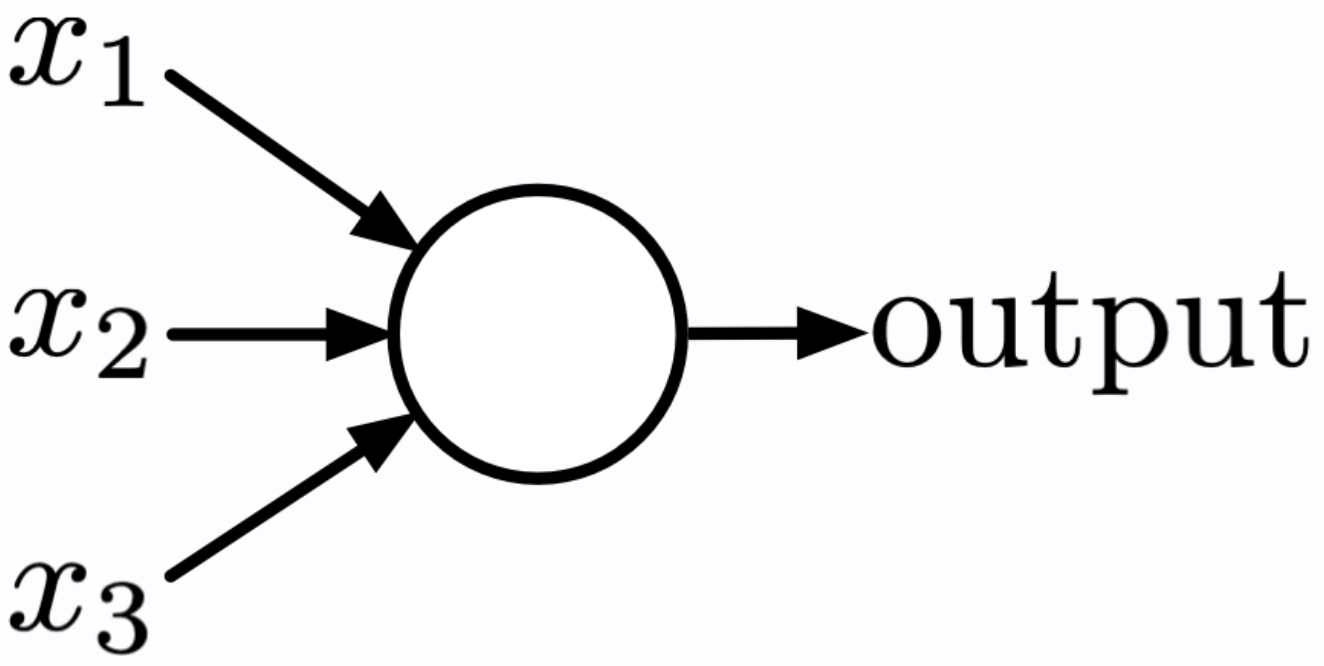
\includegraphics[scale=.4]{images/gradient_descent/perceptron.png}
    \centering
\end{figure}




Ovviamente un percettrone può esprimere concetti lineari molto semplici, ma sembra comunque plausibile che una rete complessa di percettroni possa effettuare delle decisioni più accurate. 
\begin{figure}[!h]
    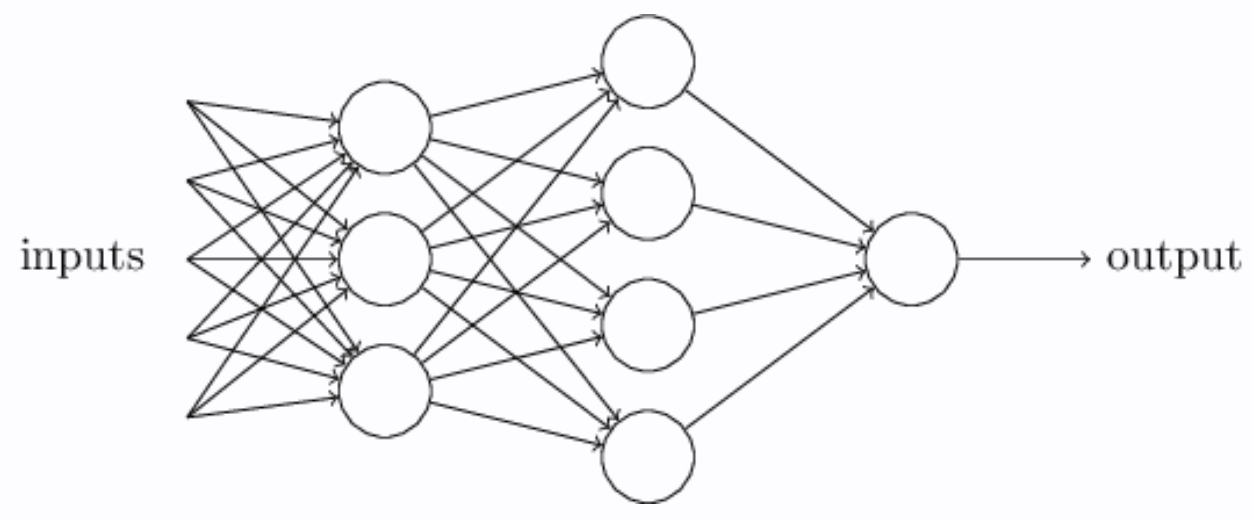
\includegraphics[scale=.4]{images/gradient_descent/perc_net.png}
    \centering
\end{figure}



Un altro modo in cui il percettrone può essere utilizzato è il calcolo delle funzioni logiche elementari. Per esempio, supponiamo di avere un percettrone con due input, ognuno con un peso di $-2$ e un bias totale di $3$.



Quale funzione booleana calcolerà questo percettrone?
\begin{figure}[!h]
    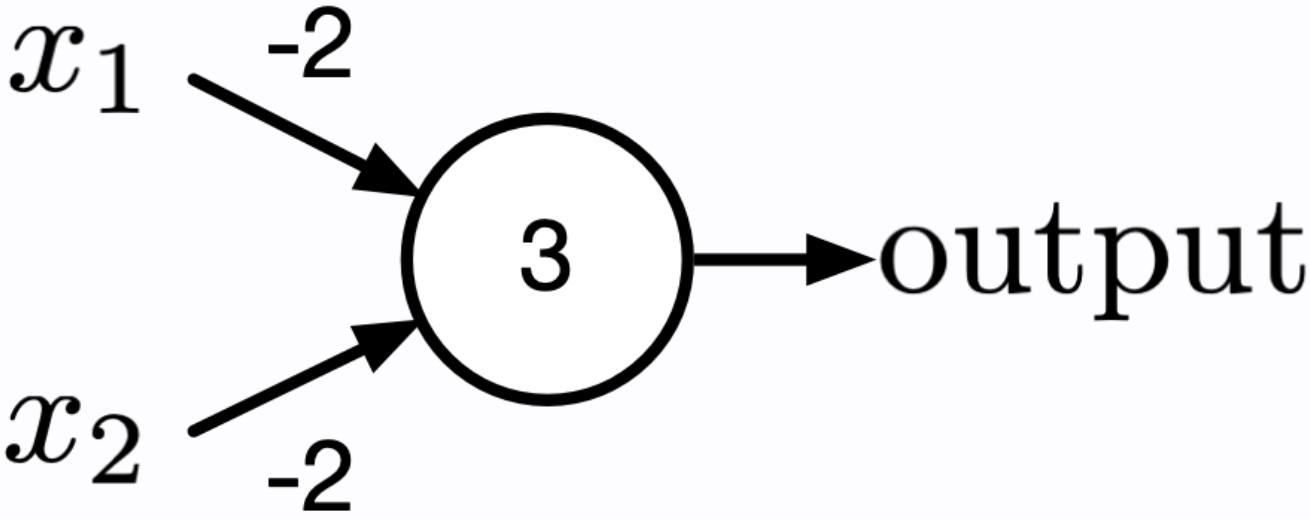
\includegraphics[scale=.4]{images/gradient_descent/perc_logic.png}
    \centering
\end{figure}
\newpage


Analizziamo come si comporta.
\begin{figure}[!h]
    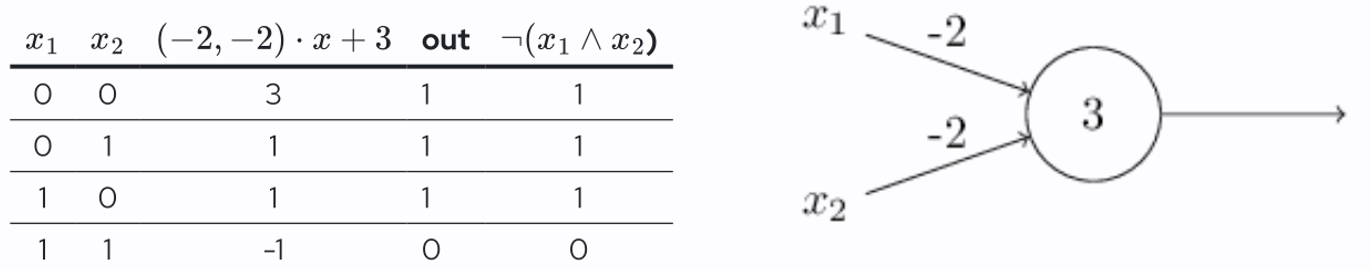
\includegraphics[scale=.7]{images/gradient_descent/nand.png}
    \centering
\end{figure}



Come sappiamo, l’esempio del NAND è particolarmente interessante perché può essere facilmente mostrato che qualsiasi altro operatore logico può essere costruito usando solamente i termini dell’operatore NAND.
Un esempio è il sommatore binario. 
\begin{figure}[!h]
    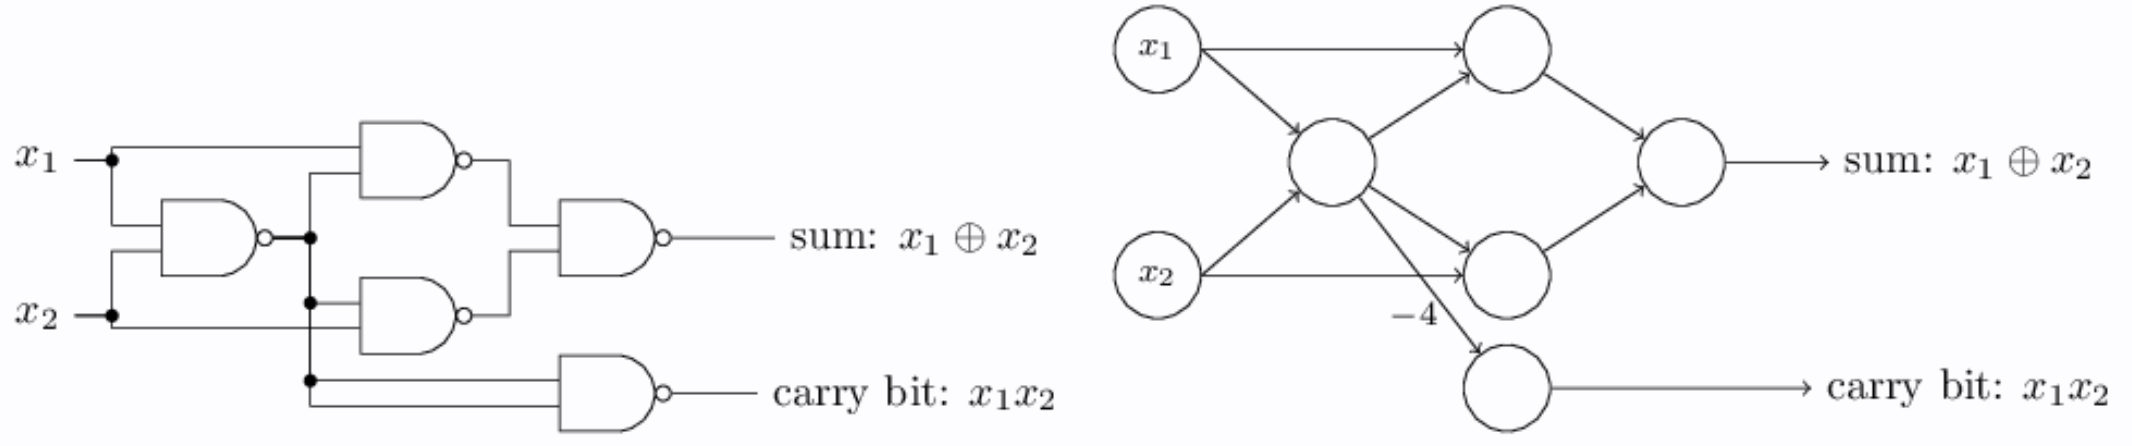
\includegraphics[width=170mm]{images/gradient_descent/bin_adder.png}
    \centering
\end{figure}



La teoria matematica delle reti neurali formalizza meglio quest’idea come la \textbf{Teoria dell’approssimazione universale}.

\newpage
\subsection{Teorema dell’approssimazione universale}
\paragraph{Def.} Una rete Feedforward con uno strato di output lineare e almeno uno strato nascosto con una qualsiasi funzione di attivazione “schiacciante” (come la funzione di attivazione del sigmoide logistico) può approssimare qualsiasi funzione misurabile di Boreal da uno spazio a dimensione finita a un altro con qualsiasi errore desiderato diverso da zero a condizione che alla rete siano fornite abbastanza unità nascoste. La derivata della rete feedforward può inoltre approssimare arbitrariamente bene le derivate della funzione.
\newline
\newline
Per i nostri scopi è sufficiente dire che qualsiasi funzione continua su un sottoinsieme chiuso e limitato è misurabile secondo Borel e quindi può essere approssimata mediante un metodo neurale rete.

\subsection{Limitazioni del teorema dell’approssimazione universale}
Sfortunatamente, nel peggiore dei casi, un numero esponenziale di unità nascoste (possibilmente con un’unita nascosta corrispondente ad ogni configurazione in ingresso che ha bisogno di essere distinta) può essere richiesto.
\newline
\newline
Questo problema è semplice da affrontare nel caso binario: il numero di possibili funzioni binarie sui vettori $v\in(0,1)^n$ è $2^{(2^n )}$ e la selezione di una di queste funzioni richiede $2^n$ bits, che generalmente richiede $O(2^n )$ gradi di libertà.
\begin{figure}[!h]
    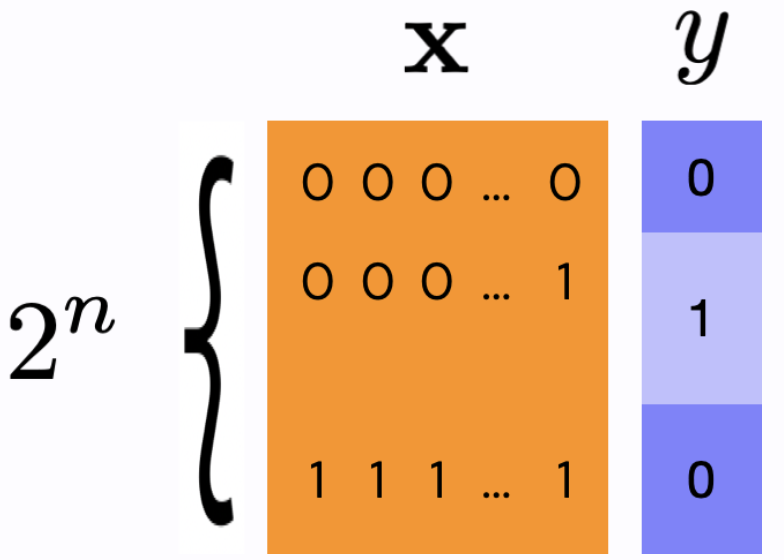
\includegraphics[scale=.8]{images/gradient_descent/limitation.png}
    \centering
\end{figure}
A questo punto sorge spontanea una domanda.


\textbf{Perché tutto ciò è così importante?}


Le risposte sono essenzialmente due:
\begin{itemize}
    \item perché le reti di percettroni possono eseguire qualsiasi tipologia di calcolo;
    \item \textbf{è possibile scrivere algoritmi in grado di imparare questi calcoli}.
\end{itemize}
\newpage
E' certamente però è molto difficile imparare qualcosa di utile utilizzando i percettroni.
\begin{figure}[!h]
    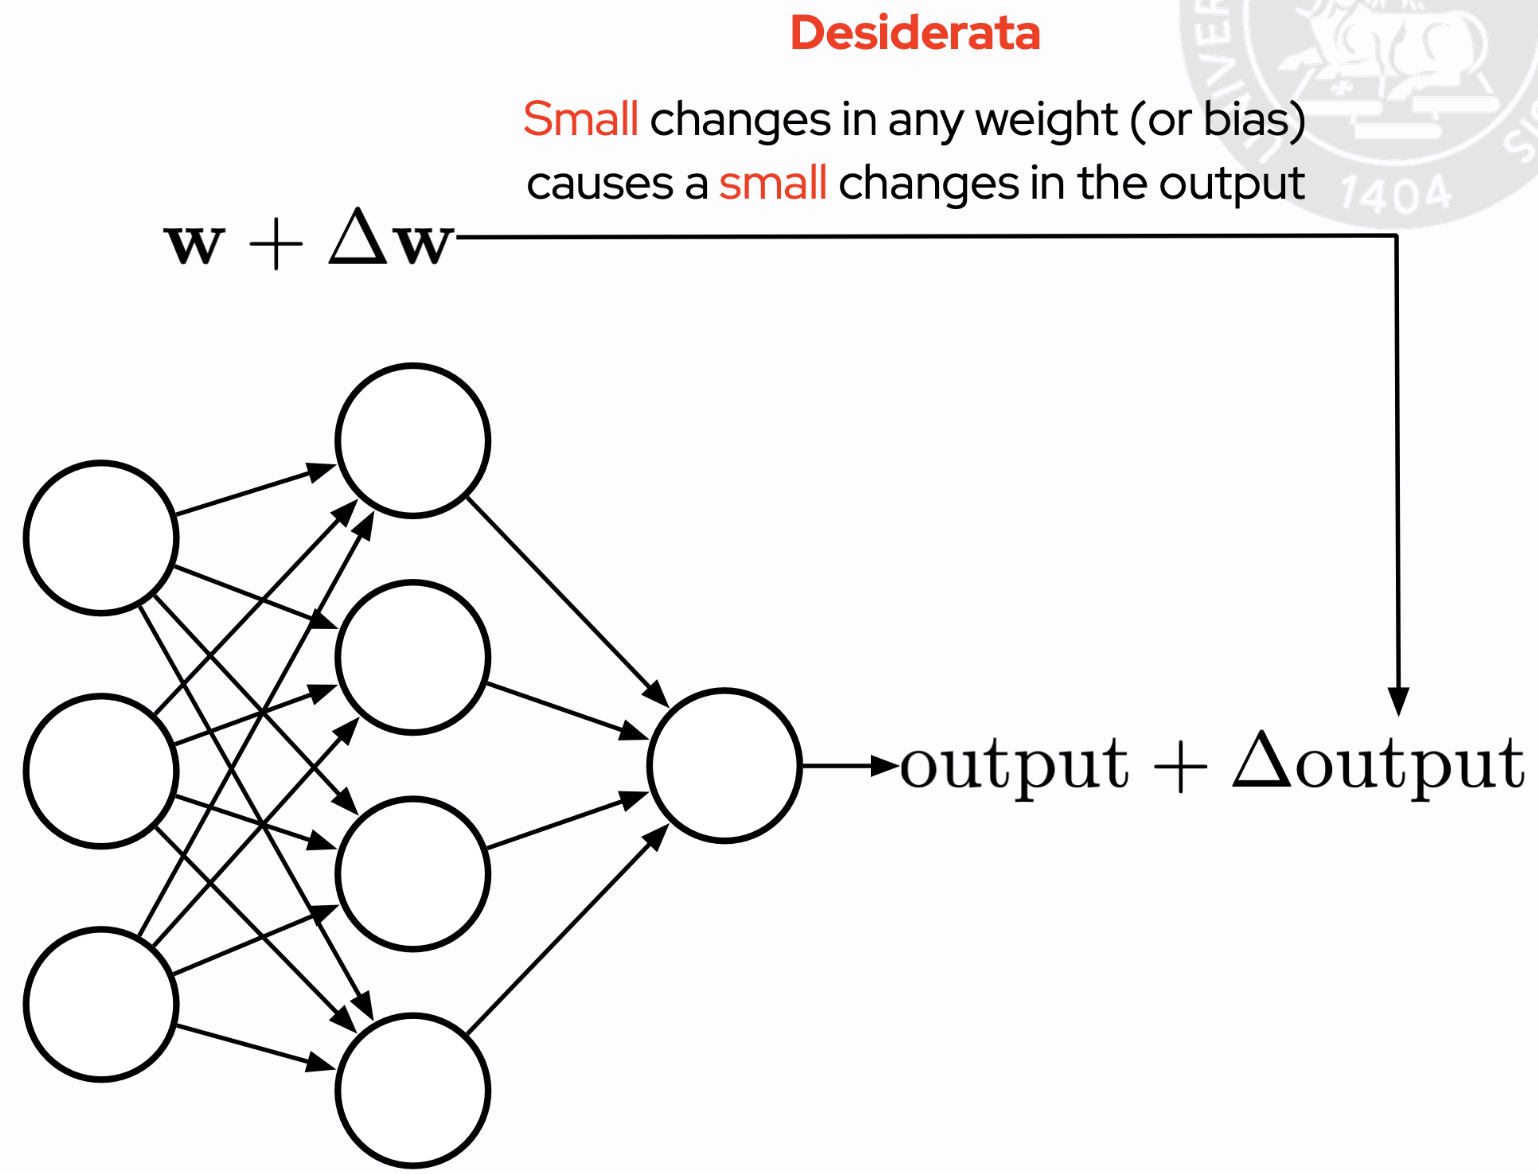
\includegraphics[scale=.3]{images/gradient_descent/sigmoid01.png}
    \centering
\end{figure}
\subsection{Neuroni sigmoide}
Un neurone sigmoide è definito come un neurone dove l’output è calcolato usando la formula: $\sigma(w\cdot x+b)$ dove $\sigma(z)=\frac{1}{(1+e^{-z})}$.
\textbf{Nota:}
\begin{itemize}
    \item gli output approssimano bene i passi della funzione quando $(w\cdot x+b)$ è estremamente grande o estremamente piccolo, ma  non cambia improvvisamente in prossimità di $0$;
    \item visto che il risultato è in $[0,1]$, gli input dei nodi interni prenderanno valori che vanno in $[0,1]$.
\end{itemize}
\begin{figure}[!h]
    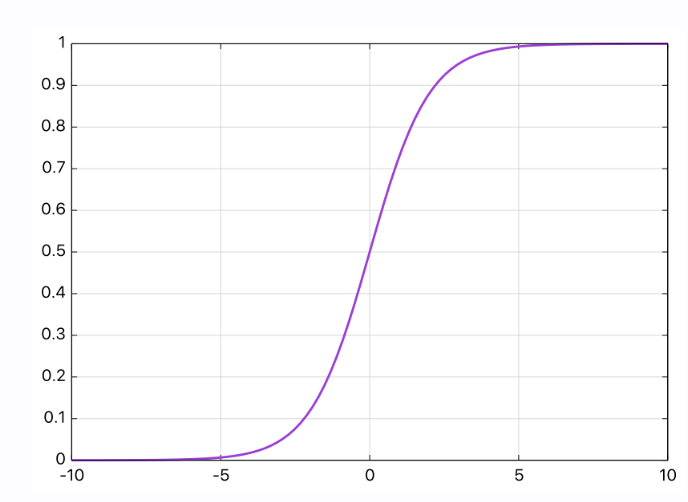
\includegraphics[scale=.6]{images/gradient_descent/sigmoid02.png}
    \centering
\end{figure}


\textbf{Ricapitolando:} è importante che la \textbf{funzione di attivazione} sia regolare poiché vorremmo controllare come varia il $\Delta output$. Il calcolo è:
\begin{equation}
    \Delta output \approx\sum_j \frac{\partial output}{\partial w_j}\Delta w_j\frac{\partial output}{\partial b}\Delta b.
\end{equation}
Abbiamo inoltre bisogno di \textbf{imporre che l'output sia differenziabile rispetto ai pesi e ai bias}.



\textbf{Nota:} l’esatta forma di $\sigma$ non è cruciale ma lo è piuttosto la sua regolarità. 


Sorge spontane la domanda: perchè $\sigma$ ha questa forma particolare? In realtà, a seconda del contesto, potrebbero essere migliori altre forme di $\sigma$.
\newpage
\section{L'architettura di una rete neurale}
\textbf{Nota:}
\begin{itemize}
    \item il livello di input non è propriamente un “livello”, semplicemente rappresenta gli input;
    \item per motivi storici, questa tipologia di architettura è chiamata \textbf{multilayer perceptron} nonostante non sia costituito da percettroni.
\end{itemize}
\begin{figure}[!h]
    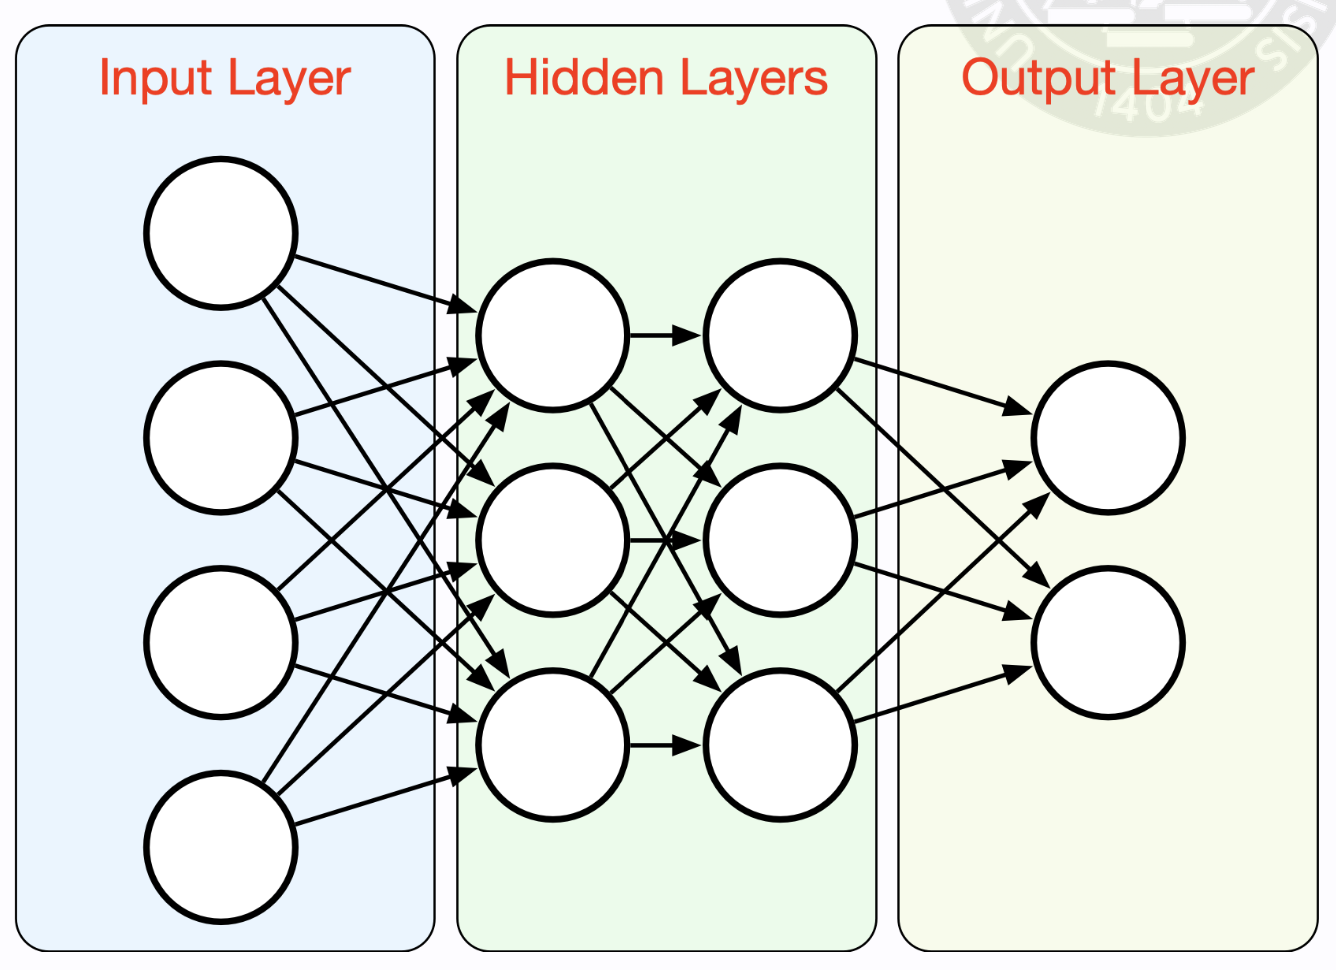
\includegraphics[scale=.35]{images/gradient_descent/architecture.png}
    \centering
\end{figure}


\paragraph{Input e output layer.} Il design dell'input e dell'output layer è spesso linerare, in particolare segue un'analisi di come sono costituiti nel caso del nostro esempio delle cifre scritte a mano.
\subsection{Il livello di input}
Rappresenteremo ogni input di training $x\in X$ con un vettore di dimensione $28\cdot 28=784$. Ogni elemento del vettore è modellato come un \textbf{neurone di input}.
\begin{figure}[!h]
    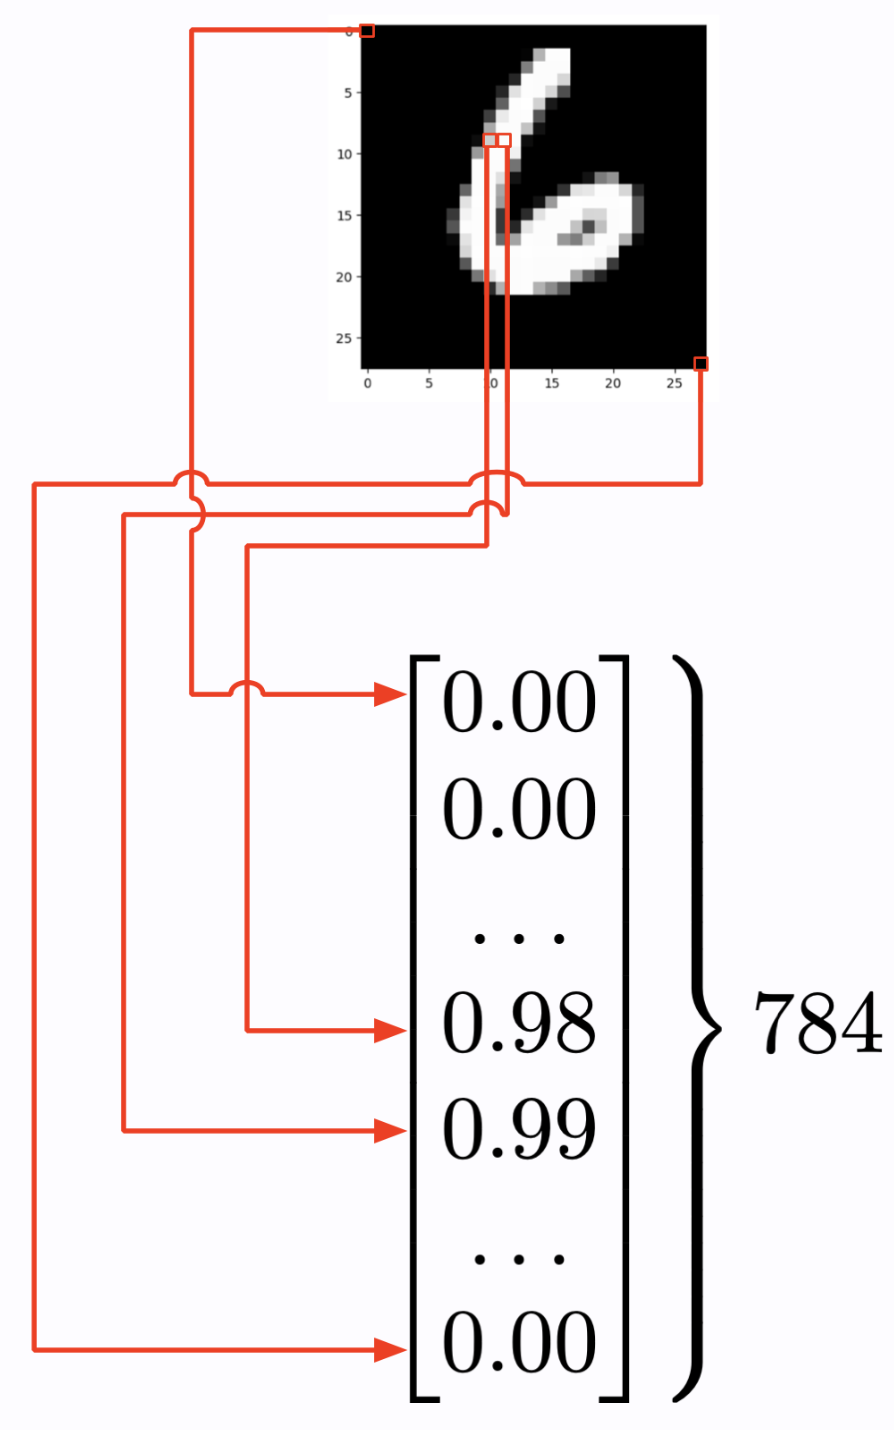
\includegraphics[scale=.35]{images/gradient_descent/input_layer.png}
    \centering
\end{figure}
\newpage
\subsection{L'output layer}
Rappresenteremo le etichette tramite $y=y(x)$ dove $y$ è un vettore avente dimensioni 10.



Per l’esempio $y(x)=(0,0,0,0,0,0,1,0,0,0)^T$ l’output sarà quello desiderato da qualsiasi rete quando $x$ è un’immagine rappresentante il valore $6$.



Ogni elemento del vettore di output sarà modellato come un \textbf{neurone di ouput}.
\begin{figure}[!h]
    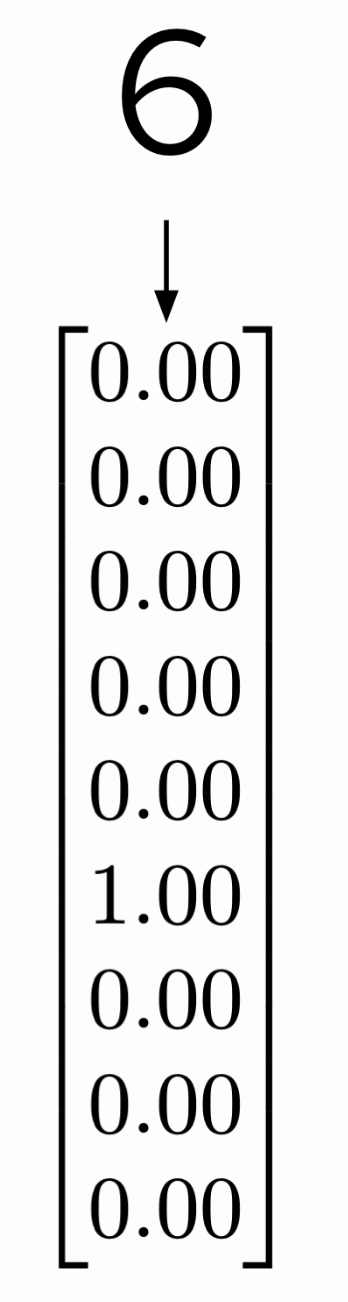
\includegraphics[scale=.35]{images/gradient_descent/output_layer.png}
    \centering
\end{figure}
\subsection{Gli hidden layer}
\textbf{Non è possibiel riassumere il design process degli hidden layer con poche semplici regole pratiche}. Infatti, i ricercatori che si occupano di reti neurali hanno sviluppato molte euristiche di design per gli hidden layer, le quali aiutano ad ottenere un comportamento desiderato da parte delle reti che si stanno utilizzando.


\textbf{Esempi:}
\begin{itemize}
    \item lan condivisione dei pesi tra neuroni permette di imparare un singolo feature detector e di applicarlo in tante location differenti;
    \item impilare i layer permette di imparare feature complesse a partire da una semplice;
    \item un grande numero di hidden units permette di imparare funzioni complesse, a patto di avere overfitting o di richiedere più dati;
    \item $\dots$
\end{itemize}

\paragraph{Il nostro esempio.} Per rappresentare le etichette utilizzando output binari sarebbero sufficienti 4 unità. Perchè allora utilizziamo $10$ cifre? \textbf{Hints:}
\begin{itemize}
    \item è un'euristica (in altre circostanze potrebbe funzionare bene);
    \item distinguere singole cifre a partire da features di immagini sembra essere più semplice di distinguerle a gruppi.
\end{itemize}
\newpage
\section{L'apprendimento con la Discesa del Gradiente}
\textbf{Vogliamo ora ideare un algoritmo di apprendimento per trovare i pesi per la nostra rete}.



Per fare questo dobbiamo definire una funzione costo che misura quanto bene la nostra rete si stia comportando e, successivamente, trovare un modo per minimizzare questa funzione costo, cioè \textbf{risolvere il problema di ottimizzazione}:
\begin{equation}
    minimize_{w,b}C(w,b)
\end{equation}
dove $C$ è una funzione dei pesi e dei biase della rete e misura quanto bene la rete performa sui dati di training $(X,y)$.
\newline
\newline
Per quantificare quanto bene il corrente set di parametri sta performando, definiamo una funzione costo:
\begin{equation}
    C(w,b)\equiv \frac{1}{2n}\sum_x \big| y(x)-z \big|^2
\end{equation}
dove $w$ denota la collezione di tutti i pesi nella rete, $b$ tutti i bias, $n$ è il numero totale di imput di training, $z$ è il vettore di output dalla rete quando $x$ è input, e la somma è su tutti gli input di training $x$.


Ovviamente $z$ dipende da $w,b,x$ e quindi può essere scritto meglio come $z_{w,b}(x)$. Lo scriveremo come $z$ per una semplificare la notazione.
\begin{figure}[!h]
    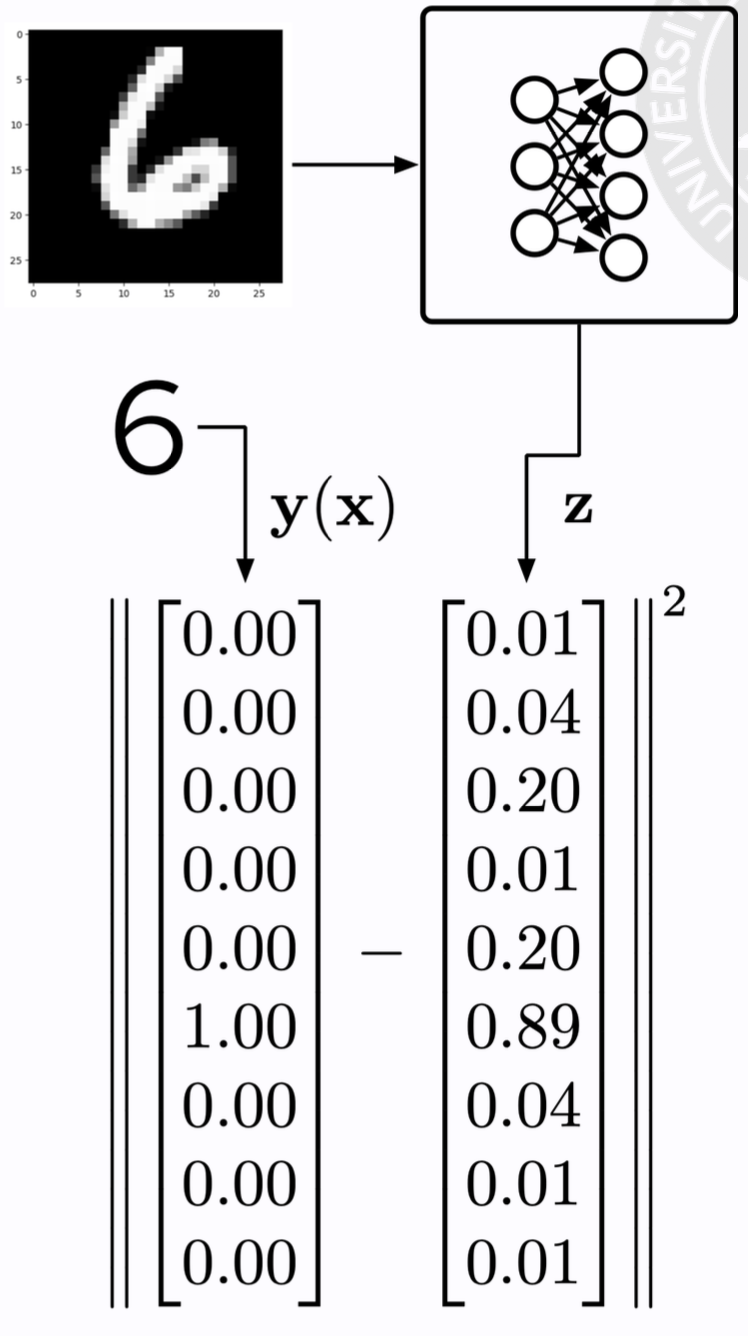
\includegraphics[scale=.5]{images/gradient_descent/cost_fun.png}
    \centering
\end{figure}
\newpage
\textbf{L'accuracy} è la misura più naturale per valutare la qualità del task di classificazione:
\begin{equation}
    A_{w,b}=\frac{1}{n}\sum_x\mathbf{I}_{y(x)=step(z)}.
\end{equation}
La funzione indicatore $\mathbf{I}_p$ restituisce $1$ se $p$ è vero e $0$ altrimenti, mentre $step(z)$ è la funzione step applicata punto per punto ad ogni elemento del vettore $z$.


\paragraph{Perché non usiamo l’accuratezza per misurare il la nostra funzione costo?} Il motivo è che l’accuratezza non è una funzione regolare dei pesi e dei bias e ciò rende difficile comprendere come cambiano i pesi e i bias al fine di incrementare le performance.


Anche tra funzioni regolari di pesi e bias, perché usiamo il costo quadratico? Non possiamo fare di meglio?


Questo è un concetto valido, ma \textbf{vedremo successivamente che ci sono altri costi che lavorano meglio in alcuni contesti}. Noi usiamo il costo quadratico perché è più semplice e funziona bene per spiegare le basi dell’apprendimento nelle reti neurali.
\newline
\newline
\textbf{Ricapitolando}, vogliamo apprendere come poter predire la cifra in un’immagine minimizzando una funzione costo:
\begin{equation}
     C(w,b)\Big( \frac{1}{2n}\sum_x \| y(x)-z \|^2 \Big)
\end{equation}
in cui l'output $z$ dipende da:
\begin{itemize}
    \item la connessione della rete;
    \item i pesi;
    \item i bias;
    \item le particolari scelte delle activation units (nel nostro esempio, sigmoidi);
    \item ecc.
\end{itemize}
Il problema è che tutto ciò è troppo complesso, quindi il nostro piano sarà:
\begin{itemize}
    \item sviluppare un metodo iterativo generale per minimizzare funzioni multivariate;
    \item sviluppare un metodo per applicarlo al caso specifico delle reti neurali.
\end{itemize}
\newpage
Consideriamo una funzione costo $C(v)$,
\begin{equation}
    C:\mathbb{R}^n\rightarrow \mathbb{R}.
\end{equation}
Per aiutarci nello sviluppo della nostra intuizione assumiamo il tempo iniziale sia $n=2$.
\textbf{Nota:} in generale sarà molto difficile individuare il minimo globale.


\begin{figure}[!h]
\centering     %%% not \center
\subfigure{\label{fig:a}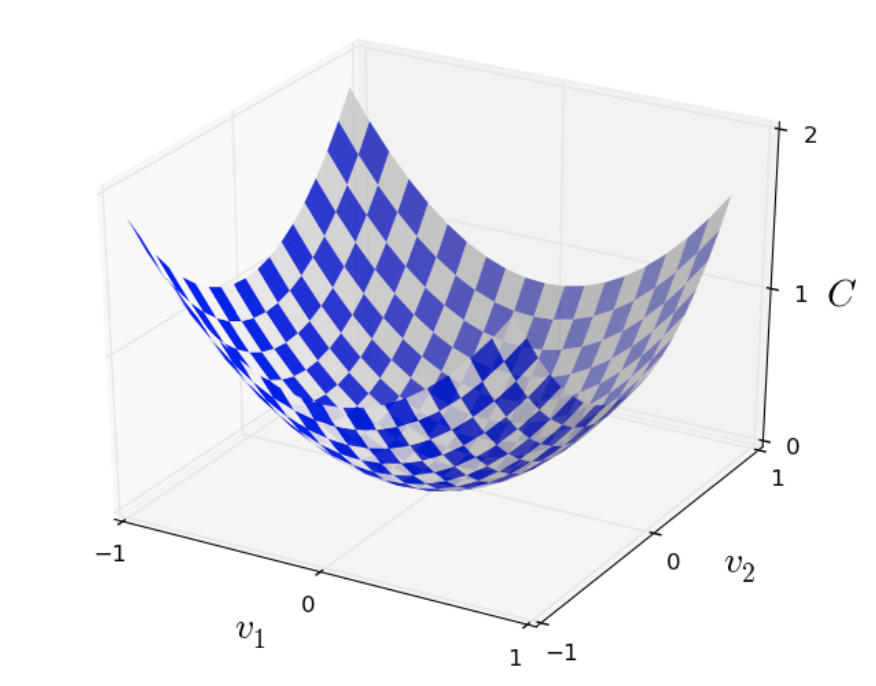
\includegraphics[scale=.5]{images/gradient_descent/minim01.png}}
\subfigure{\label{fig:b}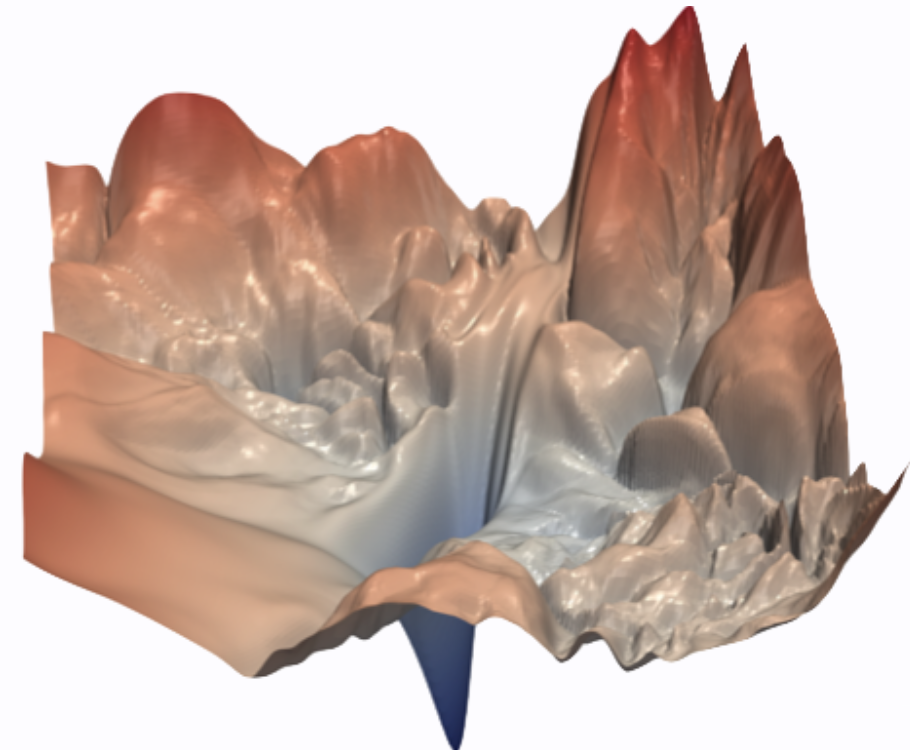
\includegraphics[scale=.5]{images/gradient_descent/minim02.png}}
\end{figure}


Nei problemi reali il numero di variabili si aggira attorno ai milioni, inoltre le dipendenze tra le variabili complicano di molto le cose.


\textbf{Usare il calcolo per trovare una una soluzione in forma chiusa semplicemente non funziona!}


Invece una soluzione migliore è immaginare il problema di minimizzazione della funzione fissando un valore sul piano $v$ e provando ad indovinare come aggiornare questa posizione per abbassare il valore della nostra funzione costo il più possibile.
\newline
\newline
Per rendere le cose più precise guardiamo cosa accade quando muoviamo le nostre variabili di una piccola quantità, diciamo  $\Delta v=(\Delta v_1,\Delta v_2)^T$.


\textbf{Il calcolo} mostra che il vettore $C$ cambia nel modo seguente:
\begin{equation}
    \Delta C\approx \frac{\partial C}{\partial v_1}\Delta v_1 + \frac{\partial C}{\partial v_2}\Delta v_2 = \nabla C \cdot \Delta v.
\end{equation}

Scegliendo $\Delta v=-\eta\nabla C$, abbiamo la garanzia che la funzione costo diminusca (a patto che lo step fatto sia sufficiente piccolo da rendere valida l’approssimazione).


Consideriamo di nuovo l'espressoine per $\Delta C$:
\begin{equation}
    \Delta C\approx \frac{\partial C}{\partial v_1}\Delta v_1 + \frac{\partial C}{\partial v_2}\Delta v_2 = \nabla C \cdot \Delta v.
\end{equation}
Settando $\Delta v=-\eta\nabla C$, avremo:
\begin{equation}
    \Delta C \approx -\eta\nabla C\cdot \nabla C = -\eta \| \nabla C \|^2 \leq 0.
\end{equation}
\newpage
La discesa del gradiente è un algoritmo  iterativo di ottimizzazione che prevede che ad ogni step muoviamo la nostra posizione corrente nella direzione opposta rispetto al gradiente:
\begin{equation}
    v'\leftarrow v-\eta\nabla C.
\end{equation}
Ciò che stiamo facendo è \textbf{diminuire la funzione errore $C$ seguendo la direzione della discesa più ripida, da qui deriva il nome}.
\begin{figure}[!h]
    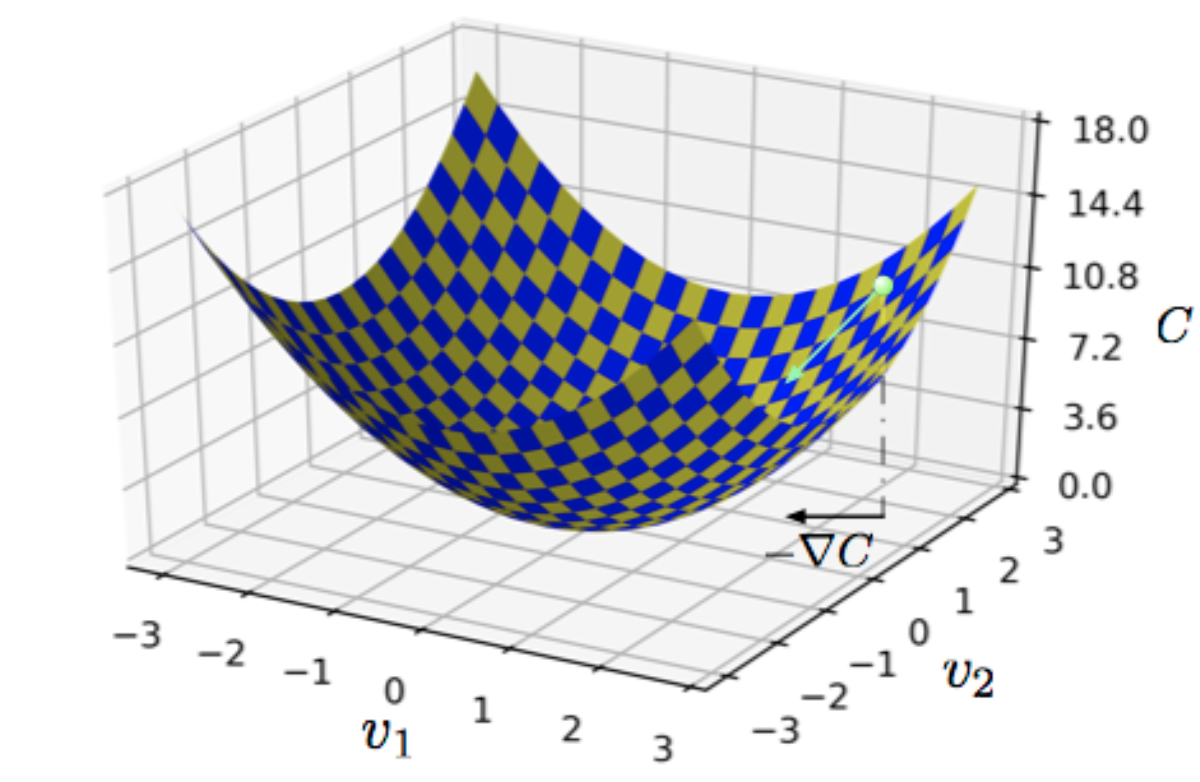
\includegraphics[scale=.5]{images/gradient_descent/grad_desc.png}
    \centering
\end{figure}


Notiamo che la scelta di $\eta$ è importante:
\begin{itemize}
    \item se è troppo grande allora l’approssimazione non sarà corretta e potremmo avere $\Delta C>0$;
    \item se è troppo piccolo l’algoritmo svolgerà piccoli step è diventerà molto lento.
\end{itemize}
\subsection{Miglioramenti della discesa del gradiente}
Perchè non ripetere l'intero ragionamento utilizzando \textbf{un'approssimazione del secondo ordine} per $\Delta C$?


Questo metodo esiste ma diventa ingestibile quando il numero di parametri cresce fino a diventare troppo grande. Il motivo è che per calcolare (per esempio) un’approssimazione del secondo ordine di $\Delta C$ dovremmo calcolare tutte le derivate parziali seconde di $C$.



Visto che il numero di derivate parziali seconde cresce quadraticamente rispetto al numero di variabili, il metodo diventa ingestibile molto velocemente.


Nonostante esistano delle tecniche per mitigare questi problemi, la discesa del gradiente (e le sue varianti) rimane il metodo più utilizzato per il training delle reti neurali.


\subsection{Applicazione della discesa del gradiente in una rete neurale}
Sostituendo $v$ con i nostri pesi $w$ e bias $b$ riusciremmo ad avere una ricetta per il training della rete neurale. Partiamo da un punto fisso e iteriamo tra i dati aggiornando ad ogni passo i pesi usando le formule:
\begin{equation}
    w'_k\leftarrow w_k-\eta\frac{\partial C}{\partial w_k},
\end{equation}
\begin{equation}
    b'_l\leftarrow b_l-\eta\frac{\partial C}{\partial b_l}.
\end{equation}
È chiaro che mancano molti dettagli nella nostra attuale formulazione corrente dell’algoritmo della discesa del gradiente.



Inoltre, \textbf{dobbiamo affrontare alcuni importanti problemi}  prima che possiamo applicare l’algoritmo in un contesto reale.



La risoluzioni di alcuni di essi è il focus del prossimo argomento.
\section{Discesa del gradiente stocastica}
Consideriamo la funzione costo $C=\frac{1}{n}\sum_xC_x$.


Il gradiente di $C$ è allora $\Delta C=\frac{1}{n}\sum_x\nabla C_x$.
Cioè per calcolare il gradiente $\nabla C$ dobbiamo calcolare il i gradienti $\nabla C_x$ separatamente per ogni input di training $x$ e poi farne una media. Solo a quel punto saremo in grado di fare uno step nella direzione suggeritaci dal gradiente. Il problema è che \textbf{quando il dataset è molto grande, questo processo diventa troppo lento}.

\paragraph{La Discesa del gradiente stocastica.} L’idea di approssimare il gradiente su tutto il dataset utilizzando un suo piccolo campione. Siano $x_1,x_2,\dots,x_m$ $m$ training input scelti randomicamente. Se $m$ è abbastanza grande, dovrebbe essere chiaro che:
\begin{equation}
    \sum_{j=1}^m\frac{\nabla C_{x_j}}{m}\approx \frac{\sum_x\nabla C_x}{n}\nabla C.
\end{equation}
Nella discesa del gradiente stocastica, viene estratto un \textbf{mini batch} di dati (un sotto insieme dei nostri dati di training) e i pesi vengono aggiornati seguendo le regole:
\begin{equation}
    w'_k\leftarrow w_k-\frac{\eta}{m}\sum_j\frac{\partial C_{x_j}}{\partial w_k},
\end{equation}
\begin{equation}
    b'_l\leftarrow b_l-\frac{\eta}{m}\sum_j\frac{\partial C_{x_j}}{\partial b_l}.
\end{equation}
Successivamente estraiamo randomicamente un altro mini batch ed effettuiamo il training con quest’ultimo. Quando verranno utilizzati tutti gli esempi diremo che avremo completato una \textbf{epoca}. A quel punto cominceremo con una nuova training epoch.







